\documentclass[../main.tex]{subfiles}

\begin{document}

    \section{Méthode} % (fold)
    \label{sec:Méthode}
    Afin de pouvoir résoudre ce problème, il faudra définir un encodage
    spécifique pour représenter un état sur un ordinateur quantique.
    Considérons un encodage d'un spin sur un qubit, soit $\ket{0}\equiv
    \ket{\downarrow}, \ket{1}\equiv\ket{\uparrow}$. Cette façon d'encoder le
    réseau dans l'ordinateur quantique permet d'avoir autant de spins que de
    qubits, soit $N=12$ au maximum ici. Un état général $\ket{\psi}$ peut être
    décrit par $2^N$ paramètres, ce qui est un peu trop compliqué à minimiser.
    On peut restreindre l'espace des états intéressants à ceux qui sont
    fortement couplés aux plus proches voisins, soit laissant seulement $4$
    connections par site, pour un réseau périodique.

    \begin{figure}[h]
        \begin{center}
            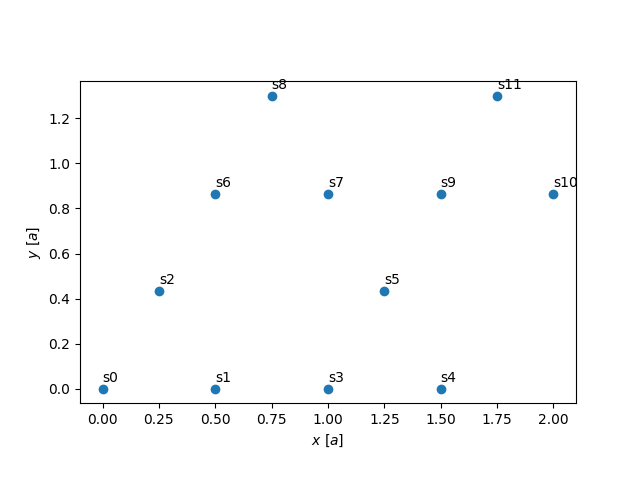
\includegraphics[width=0.95\textwidth]{../figs/reskagome.png}
        \end{center}
        \caption{Réseau kagome avec $12$ sites.}
        \label{fig:kagome}
    \end{figure}
    
    
    % section Méthode (end)

\clearpage
\end{document}
